\section{Theorie}
\label{sec:theorie}

\subsection{Berechnung der Suszeptibilität}

In Anwesenheit von Materie ändert sich ein Magnetfeld $\vec{B} = \mu_0 \vec{H}$ um die Magnetisierung
\begin{equation*}
    \vec{M} = N \mu_0 \bar{\vec{\mu}} = \mu_0 \chi \vec{H} \,,
\end{equation*}
wobei $\bar{\vec{\mu}}$ das mittlere magnetische Moment und $\chi$ die Suszeptibilität darstellt.
Dabei ist $\chi$ keine Konstante, sondern eine von $H$ und der Temperatur $T$ abhängige Größe. \\

Je nach Bereich der Suszeptibilität werden unterschiedliche Arten von Magnetismus unterschieden.
Ist die Suszeptibilität kleiner null, wird von Diamagnetismus gesprochen.
Diese Form des Magnetismus beschreibt die Induktion zum äußeren Magnetfeld entgegengerichteter magnetische Momente. \\

Hier soll der Fokus aber stärker auf dem Paramagnetismus liegen.
Der Paramagnetismus stellt, entgegen zum Diamagnetismus, keine allgemeine Eigenschaft, er findet sich nur bei
Teilchen, die einen nicht verschwindenden Drehimpuls besitzen und entsteht durch die Orientierung der an den
Drehimpuls gekoppelten magnetischen Momente zum äußeren Feld. \\

Der Gesamtdrehimpuls setzt sich jedoch nicht nur aus dem Bahndrehimpuls zusammen, sondern besteht auch dem
Elektronen- bzw. Kernspin.
Mit dem Gesamtspin $\vec{S}$ und dem Bahndrehimpuls $\vec{L}$ gilt für den Gesamtdrehimpuls
\begin{equation}
    \vec{J} = \vec{L} + \vec{S} \,.
\end{equation} \\

Die zu den Drehimpulsen gehörigen magnetischen Momente sind dabei durch

\begin{equation}
    \vec{\mu_L} = -\dfrac{\mu_\text{B}}{\hbar} \vec{L}
    \label{eq:magmomL}
\end{equation}
und
\begin{equation}
    \vec{\mu_S} = - g_\text{S} \dfrac{\mu_\text{B}}{\hbar} \vec{S}
\end{equation}
gegeben, wobei
\begin{equation*}
    \mu_\text{B} := \frac{\text{e}_0}{\text{m}_0} \hbar
\end{equation*}
das Bohrsche Magneton und $g_\text{S}$ das \textit{gyromagnetische Verhältnis des freien Elektrons}. \\

Werden nur die Beträge betrachtet, gilt
\begin{align}
    |\vec{L}| &= \sqrt{L(L + 1)} \hbar \,, \quad (L = \text{Bahndrehimpulsquantenzahl des Atoms}) 
    \label{eq:Labs} \\
    |\vec{S}| &= \sqrt{S(S + 1)} \hbar \quad (S = \text{Spinquantenzahl des Atoms})
    \label{eq:Sabs}
\end{align}
sowie
\begin{equation}
    |\vec{J}| = \sqrt{J(J + 1)} \hbar \quad (J = \text{Gesamtdrehimpulsquantenzahl des Atoms}).
    \label{eq:Jabs}
\end{equation} \\

Daraus folgt
\begin{equation}
    |\vec{\mu_\text{L}}| = \mu_\text{B} \sqrt{L(L + 1)}
    \label{eq:muLabs}
\end{equation}
und
\begin{equation}
    |\vec{\mu_\text{S}}| = \mu_\text{B} \sqrt{S(S + 1)} \,.
    \label{eq:muSabs}
\end{equation}

Aus \eqref{eq:muLabs} und \eqref{eq:muSabs} lässt sich nun das zum Gesamtdrehimpuls gehörende magnetische Moment
berechnen.
Es gilt
\begin{equation}
    |\vec{\mu_\text{J}}| = |\vec{\mu_\text{S}}| \cos \alpha + |\vec{\mu_\text{L}}| \cos\beta \,,
\end{equation}
wobei die Winkel $\alpha$ und $\beta$ wie in \autoref{fig:abb1} zu erkennen gewählt sind.

\begin{figure}
    \centering
    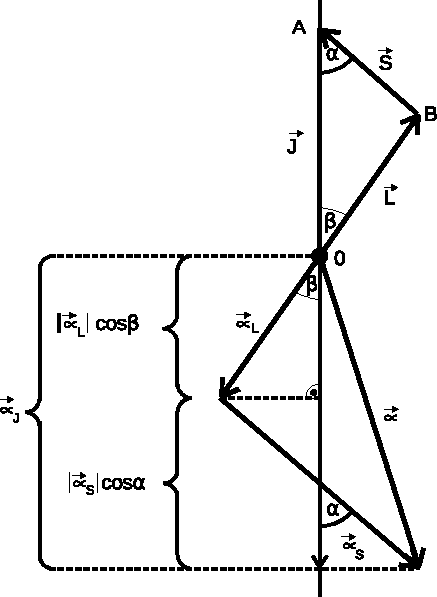
\includegraphics{figures/Abb_1.pdf}
    \caption{Vektordiagramm der magnetischen Momente\cite{ap07}.}
    \label{fig:abb1}
\end{figure}

Unter Verwendung des Cosinussatzes gilt
\begin{equation*}
    \cos\alpha = \dfrac{|\vec{J}|^2 - |\vec{L}|^2 + |\vec{S}|^2}{2|\vec{J}| |\vec{S}|}
\end{equation*}
und
\begin{equation*}
    \cos\beta = \dfrac{|\vec{J}|^2 - |\vec{L}|^2 + |\vec{S}|^2}{2|\vec{J}| |\vec{L}|} \,,
\end{equation*}
mit einigen Vereinfachung folgt dann
\begin{equation}
    g_\text{J} := \dfrac{3 J(J + 1) + {S(S + 1 - L(L + 1))}}{2 J(J + 1)} \,,
    \label{eq:lande-faktor}
\end{equation}
der Landé-Faktor des Atoms.


